\chapter{Rectificatifs : rapport de conception}

Nous avons fait très peu de changement sur la conception du projet par rapport au rapport. En effet, une bonne partie de l'application était alors déjà réalisée sous la forme du prototype utilisé lors de la phase de test en Décembre.

Le départ de quatre membres du groupe au second semestre nous a cependant beaucoup ralentit. Nous avons pu voir qu'il est bien souvent difficile de reprendre le travail effectué par d'autres personnes. Il a d'abord fallu reprendre le code déjà effectué pour le corriger et le commenter de façon plus détaillée.

Après nous êtres assurés d'avoir une base était solide et fonctionnelle, nous avons pu continuer le développement sans rencontrer de problème majeur. 

Des changements notables concernent la base de donnée. Nous avons parfois du ajouter quelques attributs à certaines entités pour permettre l'implémentation de fonctionnalités avancées (ajout d'un attribut date aux fichier mis en ligne par exemple, etc). La nouvelle base de donnée est représentée sur la figure \ref{bdd}. Nous avons aussi supprimé l'attribut "state" des utilisateurs, car nous ne différencions plus les différentes phases de cette manière (voir partie 3.2).

Enfin, nous avons du ajouter un élément à l'architecture du projet afin de gérer le passage des année. Tout cela est effectué grâce à l'entité "CronTask" qui s'exécute au début de chaque année scolaire.


\begin{figure}
	\centering
	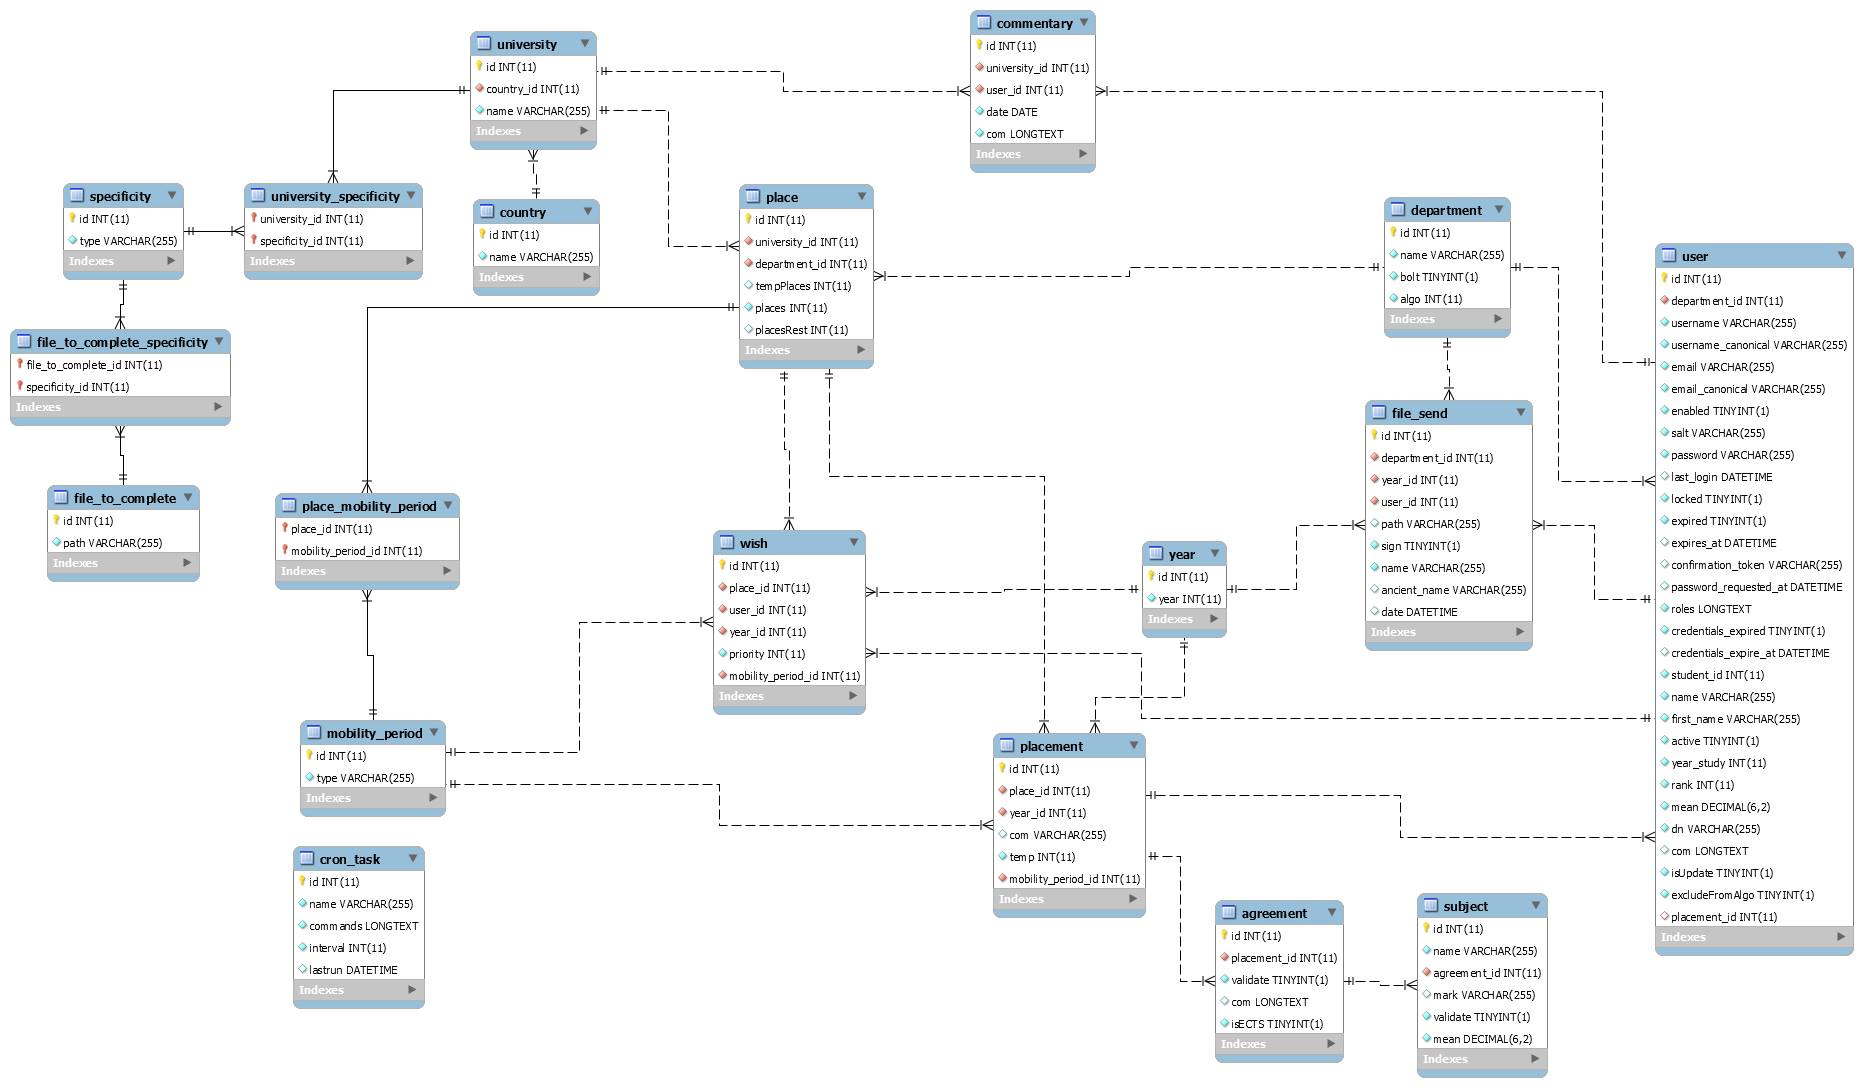
\includegraphics[angle=90,scale=0.35]{images/screen_bdd.png}
	\caption{Nouvelle base de données}
	\label{bdd}
\end{figure}

